\documentclass[english]{sbc2025}%

\usepackage[misc,geometry]{ifsym}
\usepackage{aas_macros}
\usepackage[bottom]{footmisc}
\usepackage{tabularray}
\usepackage{afterpage}
\usepackage{url}
\usepackage{pifont}
\usepackage{booktabs}
\usepackage{multirow}
\usepackage{tikz}
\usetikzlibrary{arrows.meta,positioning,fit,backgrounds}

\setcitestyle{square}

\definecolor{engtitle}{rgb}{0.5,0.5,0.5}
\definecolor{orcidlogo}{rgb}{0.37,0.48,0.13}
\definecolor{unilogo}{rgb}{0.16, 0.26, 0.58}
\definecolor{maillogo}{rgb}{0.58, 0.16, 0.26}
\definecolor{darkblue}{rgb}{0.0,0.0,0.0}
\hypersetup{colorlinks,breaklinks,
            linkcolor=darkblue,urlcolor=darkblue,
            anchorcolor=darkblue,citecolor=darkblue}

% ---------------------------------------------------------------------
% Drafting macros -- remove before submission
%   \tbd{...}  : content that depends on results still being generated
%   \chk{...}  : statement/parameter to be confirmed by the coauthors
% ---------------------------------------------------------------------
\newcommand{\tbd}[1]{\textcolor{red}{[TBD: #1]}}
\newcommand{\chk}[1]{\textcolor{orange!80!black}{[CHECK: #1]}}
\newcommand{\figplaceholder}[2]{%
  \fbox{\parbox[c][#1][c]{0.95\columnwidth}{\centering\small\textcolor{red}{#2}}}}
\newcommand{\cmark}{\ding{51}}
\newcommand{\xmark}{\ding{55}}

% Notation
\newcommand{\Tb}{T_{\mathrm{b}}}
\newcommand{\Cb}{C_{\mathrm{b}}}
\newcommand{\Cn}{C^{\max}_{\mathrm{node}}}
\newcommand{\Lt}{L^{95}_{\mathrm{tx}}}
\newcommand{\Th}{\Theta}
\newcommand{\Ut}{U}
\newcommand{\nmax}{n_{\max}}
\newcommand{\Kn}{K_{\mathrm{node}}}
\newcommand{\tbdc}{\textcolor{red}{?}} % pending table cell

\jid{iSys}
\jtitle{iSys - Journal of Information Systems, 202X, XX:1}
\issn{1984-2902}
\doi{10.5753/isys.202X.XXXXXX}
\copyrightstatement{This work is licensed under a Creative Commons Attribution 4.0 International License}
\jyear{202X}

\category{Research Paper}

\title[Sizing Byzantine Consensus for REDD+ Registries]{Sizing Byzantine Consensus for Blockchain-Based REDD+ Registries: Governance, Demand, and Feasibility Frontiers}

% THE ORCID IS MANDATORY FOR EACH AUTHOR -- author order to be confirmed
\author[Freire et al. 202X]{
\affil{\textbf{Fabricio Rodrigues Freire}~\orcidlink{0000-0000-0000-0000}~\textcolor{blue}{\faEnvelopeO}~~[{Universidade de Bras\'ilia}~|\href{mailto:fabriciorfreire@gmail.com}{~{\textit{fabriciorfreire@gmail.com}}}~]}

\affil{\textbf{Marcela Ceschim Caburl\~ao}~\orcidlink{0009-0003-7911-8166}~~[{Universidade Federal do ABC}~|\href{mailto:xxx@ufabc.edu.br}{{\textit{xxx@ufabc.edu.br}}}~]}

\affil{\textbf{Carlo Kleber da Silva Rodrigues}~\orcidlink{0000-0003-1231-6953}~~[{Universidade Federal do ABC}~|\href{mailto:xxx@ufabc.edu.br}{{\textit{xxx@ufabc.edu.br}}}~]}
}

\begin{document}

\begin{frontmatter}

\maketitle

\begin{mail}
\chk{Corresponding author postal address.}
\end{mail}

\begin{abstract-en}
Blockchain-based carbon credit registries have been proposed to provide integrity and traceability to REDD+ projects, and Brazilian Law 15,042/2024 opens the prospect of a national registry. The viability of Byzantine consensus at this scale, however, has been discussed with models that size the validator set by forest area and estimate consensus traffic in closed form. This work investigates under which conditions each family of consensus protocols remains viable for a national registry and which constraint becomes binding first. The number of validators is treated as a governance scale, separated from the market scale that determines demand, and demand is modeled from the periodic reconciliation structure of the regulated market. Admissible protocols are selected from domain requirements and evaluated on the JABS simulator, with packet-level traffic measurement and Byzantine validators, in a factorial experiment whose analysis protocol is fixed before the main battery. Elasticities with respect to both scales are estimated by metamodels validated outside the fitting range, and interactions are tested by ANOVA with robustness checks. \tbd{Measured elasticities, binding constraint per regime and feasibility frontiers.} \tbd{Confirm or refute the hypothesis that viability depends more on governance design than on transaction volume.} In either case, the resulting frontiers indicate how many validators a registry can accommodate for each demand level.
\end{abstract-en}

\begin{keywords}
Blockchain, Byzantine Consensus, Scalability, REDD+, Carbon Registry, Analysis of Variance
\end{keywords}

\begin{dates}
\noindent{\sffamily\textbf{Received:}} DD Month YYYY~~~$\bullet$~~~
{\sffamily\textbf{Accepted:}} DD Month YYYY~~~$\bullet$~~~
{\sffamily\textbf{Published:}} DD Month YYYY
\end{dates}

\end{frontmatter}

% =====================================================================
\section{Introduction}
\label{sec:intro}
% =====================================================================

Blockchain technology has received a great deal of attention in the past few years since it can address the issues of trust, traceability and double counting in forest carbon markets, without necessarily relying on centralized intermediaries \citep{Howson2019ncc,Kotsialou2022}. Owing to this fact, several reported contributions have investigated the use of distributed ledgers in the governance of carbon markets and in the management of credits generated by projects of Reducing Emissions from Deforestation and Forest Degradation (REDD+) (see for instance \citep{Howson2019geoforum,Kotsialou2021,Marke2022,Vilkov2023,He2022} and references therein). In Brazil, this discussion acquired an institutional dimension with Law 15,042/2024, which established the Brazilian Emissions Trading System (SBCE), with a central registry operated by a managing body, periodic reporting and reconciliation obligations for regulated operators, and explicit mechanisms against the double counting of jurisdictional credits \citep{Lei15042}. As a result, the question of whether a national-scale registry could be supported by Byzantine consensus has become concrete.

The available quantitative evaluations do not answer this question. The works of \citet{Caburlao2025reic} and \citet{Caburlao2026clei} compared, by means of the JABS simulator \citep{Yajam2023}, the block finalization time and traffic of three operating REDD+ projects, Ambify \citep{Ambipar2021}, MCO2 \citep{Moss2020} and TreeCycle \citep{GlobalTree2019}, and showed that these indicators are largely determined by the underlying consensus mechanism. In these studies, the number of nodes was sized by the monitored forest area, at a ratio of one node per $1{,}000$ hectares, which is adequate for comparing individual projects. When extrapolated to the national scale, however, this parameterization leads to validator sets of about $10^{5}$ nodes, for which no known Byzantine protocol is viable. Furthermore, in the version of the simulator used in the development of the Arq-REDD+ architecture \chk{cite the Arq-REDD+ reference once published}, the consensus traffic of pBFT is obtained from a closed-form estimate proportional to the number of nodes, rather than measured \chk{confirm whether previously disseminated results used this estimate}. A linear estimate cannot reveal whether the communication overhead becomes the binding constraint, since, in the normal case of pBFT, the number of messages per block grows with the square of the number of nodes \citep{Castro1999}. Therefore, national-scale viability remains an open question, which cannot be answered by yet another comparison among algorithms.

The present work builds upon a simple observation with direct consequences for the design of the registry: in a regulated registry, the number of validators is not a territorial quantity but a governance decision, bounded by the number of accountable institutions (managing body, federative units, accredited verifiers); the transaction demand, in turn, is a market quantity, determined by the number of operators and by the temporal structure of the reconciliation obligations. The two scales affect consensus in different ways. While the communication cost of each consensus round grows with the number of validators, the transaction volume is aggregated into blocks and mainly affects the block size and the link occupancy. To the best of the authors' knowledge, the viability of blockchain-based carbon registries has not been analyzed by separating these two scales, nor on the basis of a demand derived from the structure of the regulated market.

Motivated by the above, this work investigates under which conditions each family of consensus protocols remains viable for a national registry and which constraint becomes binding first. The working hypothesis, to be confirmed or refuted by the experiments, is that viability is more sensitive to the governance scale than to the market scale. The main contributions are as follows:

\begin{itemize}
\item The registry sizing problem is formulated in two independent scales, governance ($n$ validators) and market (demand $\lambda$), and the effect of coupling $n$ to the forest area is quantified with packet-level traffic measurement.
\item A demand model is derived from the periodic reconciliation structure of the SBCE, with closed-form parameters for a Markov-modulated Poisson process, instead of assuming stationary Poisson arrivals.
\item The evaluated protocols are selected from domain requirements (deterministic finality, accountable validators, Byzantine tolerance and low energy cost), and the role of each retained protocol is made explicit.
\item Elasticities of traffic, latency and link occupancy with respect to both scales are estimated, with Byzantine validators, by metamodels validated outside the fitting range, and feasibility frontiers $\nmax(\lambda)$ that identify the binding constraint in each regime are derived.
\end{itemize}

The remainder of the paper is organized as follows: Section~\ref{sec:background} presents the theoretical background and Section~\ref{sec:related} discusses the related work. Section~\ref{sec:model} defines the registry requirements, the two scales, the demand model and the feasibility criteria. Section~\ref{sec:method} details the experimental design and the analysis procedure. Numerical results and insightful discussions are provided in Section~\ref{sec:results}. Finally, concluding remarks are provided in Section~\ref{sec:conclusion}.

% =====================================================================
\section{Theoretical Background}
\label{sec:background}
% =====================================================================

\subsection{Carbon Markets, REDD+ and the SBCE}

Carbon markets allow the emissions avoided or removed by an activity to be quantified, certified and traded as credits, where each credit typically corresponds to one tonne of carbon dioxide equivalent \citep{Aguiar2018}. REDD+ projects generate credits by reducing deforestation and forest degradation with respect to a reference scenario, which renders them particularly relevant for Brazil \citep{Aguiar2018,Neves2025}. The credibility of these projects depends on the measurement, reporting and verification (MRV) process, historically characterized by opaque data, high transaction costs, manual procedures and dependence on intermediaries, which renders the market vulnerable to fraud and double counting \citep{Kotsialou2022,Howson2019geoforum,Caburlao2026fsi}.

Law 15,042/2024 established the SBCE, in which operators with annual emissions above $10{,}000$~tCO$_2$e must submit a monitoring plan and emission reports, and those above $25{,}000$~tCO$_2$e must, in addition, periodically reconcile their obligations by holding SBCE assets equivalent to their net emissions \citep{Lei15042}. The system foresees a central registry managed by a managing body, the integration of credits verified under registered methodologies, and jurisdictional REDD+ programs at national or state level. From the computational standpoint, two aspects of this structure are decisive: the set of entities that may validate records is institutionally bounded, and operations tend to concentrate around reconciliation deadlines.

\subsection{Blockchain Technology}

A blockchain is a distributed ledger in which transactions are grouped into blocks that are cryptographically chained and replicated among the participants of a peer-to-peer network \citep{Nakamoto2008}. Its properties of decentralization, immutability and transparency make it suitable for recording the issuance, transfer and retirement of carbon credits, as well as for their tokenization \citep{Vilkov2023,Kotsialou2021}. From the security standpoint, the guarantees of a blockchain-based registry are commonly analyzed in terms of the confidentiality, integrity and availability triad \citep{Aminzade2018,Tchernykh2019,Rashidibajgan2024}, together with application-layer risks such as smart contract vulnerabilities \citep{GhiyamiPour2025}, the trustworthiness of the oracles that bring MRV data into the ledger \citep{Rahman2023}, and on-chain governance \citep{Esposito2025}. The selection of a distributed ledger technology therefore involves trade-offs between performance, security and decentralization \citep{Werth2023,Rodrigues2024}.

\subsection{Consensus Protocols and Communication Complexity}

Consensus protocols can be classified into proof-based and voting-based families \citep{Xiao2020,Bamakan2020}. In the Nakamoto consensus based on proof of work (PoW), the right to append a block is obtained through the expenditure of computational resources, and finality is probabilistic \citep{Nakamoto2008}. In proof of stake (PoS), this right is proportional to the stake of the validators, and finality can be provided by an overlay such as Casper FFG, which finalizes blocks at periodic checkpoints and tolerates less than one third of malicious stake \citep{Buterin2017}. Proof of staked authority (PoSA), modeled as Parlia in JABS, combines a restricted set of authorized validators with stake-based selection \citep{Caburlao2026clei}.

Voting-based protocols derive from the Byzantine fault tolerance (BFT) state machine replication literature \citep{Vukolic2015}. pBFT \citep{Castro1999} guarantees deterministic finality as long as at most $f$ out of $n \geq 3f+1$ validators are faulty. In its normal, failure-free case, each block requires a pre-prepare phase, in which the leader sends $n-1$ messages, and two all-to-all broadcast phases (prepare and commit), which results in a number of messages per block of the order of
\begin{equation}
M_{\mathrm{pBFT}}(n) \approx 2n^{2},
\label{eq:mpbft}
\end{equation}
while each node sends and receives $O(n)$ messages. Tendermint \citep{Buchman2018} adopts a rotating proposer and gossip-based vote propagation, while preserving two all-to-all voting rounds. HotStuff \citep{Yin2019}, in turn, concentrates the votes at the leader and uses threshold signatures, which reduces the total number of messages in the normal case to $O(n)$; however, the leader still sends and receives $O(n)$ messages per phase. This distinction is central to this work: a protocol may have a linear total cost and still present a node whose link becomes the binding constraint.

The normal case does not settle the question. \citet{Dolev1985} proved that deterministic Byzantine agreement protocols require $\Omega(n + f^{2})$ messages in executions with up to $f$ faulty processes, which, for $f$ proportional to $n$, amounts to $\Omega(n^{2})$. Thus, even a protocol that is linear in the normal case, such as HotStuff, incurs a quadratic cost when successive faulty leaders force view changes. For this reason, the viability assessment must include Byzantine validators, and not only the normal case. As a structural alternative, hierarchical architectures run consensus within local groups and only representatives take part in the global consensus \citep{Amir2010}.

\subsection{Performance Evaluation of Computer Systems}

According to \citet{Jain1991}, a systematic performance study comprises the statement of goals and system boundaries, the selection of metrics, the characterization of the workload, the selection of factors and levels, the design of experiments and the analysis of data. The ANOVA allows effects and interactions to be tested and the variation of a response to be allocated among the factors, their interactions and the experimental error \citep{Jain1991,Montgomery2017}. The share of variation attributed to each factor, however, depends on the range of the chosen levels, and should not be interpreted as intrinsic importance when the factors have arbitrary ranges. When the evaluation is conducted by simulation, the experimental error is controlled through independent replications and the removal of the initial transient \citep{Law2015}, and regression models fitted to the results (metamodels) should only be used for extrapolation after validation at points not used in the fit \citep{Kleijnen2015}. In this work, this methodology supports the evaluation of an artifact in the design science paradigm \citep{Hevner2004}: a sizing method for carbon registries, composed of the requirement-based protocol selection, the demand model, the feasibility frontiers and the recommendation rule.

% =====================================================================
\section{Related Work}
\label{sec:related}
% =====================================================================

The potential of blockchain for REDD+ has been examined from the economic, institutional and environmental standpoints \citep{Howson2019geoforum,Kotsialou2021,Kotsialou2022,Marke2022,Pak2021}, and systematic reviews have mapped its applications in carbon markets and in forestry \citep{Vilkov2023,He2022}. In the Brazilian context, \citet{Aguiar2018} analyzed the voluntary forest carbon market, and \citet{Neves2025} investigated blockchain in the jurisdictional REDD+ system of the state of Acre. More recently, \citet{Caburlao2026fsi} identified a scarcity of empirical validation and of detailed technical architectures in this field.

Evaluations of consensus mechanisms are numerous and mostly comparative. \citet{Bamakan2020} organized performance evaluation criteria for consensus algorithms, \citet{Werth2023} examined platforms in the light of the scalability, security and decentralization trilemma, and \citet{Shen2025} and \citet{Shaikh2025} proposed reviews and comparative frameworks. Simulation-based comparisons were conducted for network sharing \citep{Zeydan2026} and for energy trading in microgrids \citep{Bhavana2025}. These works rank protocols under workloads and scales fixed by the authors, but do not derive the workload or the size of the validator set from the application domain.

In the REDD+ domain, \citet{Caburlao2025reic,Caburlao2026clei} compared operating projects by simulation, with traffic measured in the simulator, confidence intervals and sensitivity analysis, considering the PoS and PoSA mechanisms of these projects. \citet{Bastos2026} evaluated a permissioned architecture on Hyperledger Besu for REDD+ credits in the Amazon through load tests with up to $250$ concurrent users. Outside the carbon domain, \citet{Rodrigues2021} analyzed blockchain-integrated architectures for Internet of Things transactions, and \citet{Rodrigues2024} studied the selection of distributed ledger technologies.

However, none of the above-cited works (i) separates the governance scale from the market scale, (ii) derives the demand from the obligation structure of a regulated market, (iii) includes classical BFT protocols with packet-level measured traffic and Byzantine validators in the context of carbon registries, and (iv) validates scaling laws outside the fitting range to estimate viability limits. Table~\ref{tab:related} summarizes these differences.

\begin{table*}[!ht]
\caption{Comparison with related works. Scl.: separates governance and market scales; Dem.: domain-derived demand; BFT: includes classical BFT protocols with measured traffic and Byzantine validators; Frt.: feasibility frontier validated outside the fitting range.}
\label{tab:related}
\centering
\small
\begin{tabular}{@{}lcccccc@{}}
\hline\hline
Work & REDD+ & Simulation & Scl. & Dem. & BFT & Frt. \\
\hline
\citet{Bamakan2020}      & --     & --     & --     & --     & --     & -- \\
\citet{Zeydan2026}       & --     & \cmark & --     & \chk{} & \chk{} & -- \\
\citet{Bastos2026}       & \cmark & --     & --     & \chk{} & \chk{} & -- \\
\citet{Caburlao2026clei} & \cmark & \cmark & --     & --     & --     & -- \\
This work                & \cmark & \cmark & \cmark & \cmark & \cmark & \cmark \\
\hline\hline
\end{tabular}
\end{table*}

% =====================================================================
\section{Requirements, Scales and Feasibility Criteria}
\label{sec:model}
% =====================================================================

\subsection{Registry Requirements and Protocol Selection}

The evaluated protocols are selected from four requirements that stem from the legal and institutional nature of a carbon registry:

\begin{itemize}
\item \textbf{R1 -- Deterministic and immediate finality.} The transfer and retirement of a credit produce legal and accounting effects; probabilistic finality, or finality reached only after several periods, would reopen a reversal window and, consequently, the possibility of double counting.
\item \textbf{R2 -- Identified and accountable validators.} In the SBCE, the central registry is managed by a managing body and the other participants are regulated or accredited entities \citep{Lei15042}; a validator set open to any stakeholder is not compatible with this structure.
\item \textbf{R3 -- Byzantine tolerance with a known threshold.} Proponents, verifiers and buyers have conflicting interests, so that the registry must tolerate malicious validators up to an explicit threshold.
\item \textbf{R4 -- Low energy cost.} A climate policy instrument should not depend on a mechanism whose energy cost grows with the desired security.
\end{itemize}

Table~\ref{tab:req} confronts the protocol families with these requirements. PoW violates R1, R2 and R4 and is therefore excluded. The classical BFT protocols meet all requirements, and each is retained for a specific reason: pBFT is the protocol adopted by Arq-REDD+ and represents the quadratic reference cost; HotStuff tests the hypothesis that reducing the total normal-case cost to $O(n)$ shifts the feasibility frontier; and Tendermint represents the BFT used in production in consortium networks. PoS only partially meets R1 and R2, since Casper FFG finality is reached only at periodic checkpoints and the validator set is open to stakeholders \citep{Buterin2017}. PoSA meets R2 but only partially meets R1, since finality depends on additional voting rounds of the authorized validators \chk{confirm how Parlia finality is modeled in JABS}. Both are nevertheless retained as external validity anchors, since they are the mechanisms of the operating REDD+ projects (MCO2 and Ambify) and allow the results of this work to be related to those of \citep{Caburlao2026clei}. This exception is deliberate and does not extend to the final recommendation, which requires full compliance with R1--R4.

\begin{table}[!ht]
\caption{Fulfillment of the registry requirements by protocol families (\cmark: met; $\circ$: partially met; \xmark: not met).}
\label{tab:req}
\centering
\footnotesize
\setlength{\tabcolsep}{3pt}
\begin{tabular}{@{}lccccl@{}}
\hline\hline
Protocol & R1 & R2 & R3 & R4 & Role in the study \\
\hline
PoW        & \xmark  & \xmark  & $\circ$ & \xmark & excluded \\
PoS        & $\circ$ & $\circ$ & \cmark  & \cmark & anchor (MCO2) \\
PoSA       & $\circ$ & \cmark  & \cmark  & \cmark & anchor (Ambify) \\
pBFT       & \cmark  & \cmark  & \cmark  & \cmark & $O(n^2)$ reference \\
Tendermint & \cmark  & \cmark  & \cmark  & \cmark & production BFT \\
HotStuff   & \cmark  & \cmark  & \cmark  & \cmark & $O(n)$ hypothesis \\
\hline\hline
\end{tabular}
\end{table}

\subsection{Governance Scale and Market Scale}

As shown in Fig.~\ref{fig:system}, we consider a registry with $n$ validators, of which $f = \lfloor \phi n \rfloor$ behave in a Byzantine manner, where $\phi$ is the Byzantine fraction and $f$ must satisfy the tolerance threshold of each protocol ($n \geq 3f+1$ for the BFT protocols and Casper FFG). The transaction demand has rate $\lambda(t)$ and is generated by the operators and by the participants of the voluntary market.

The size of the validator set is treated as a governance variable. In a configuration in which each of the 27 federative units, the managing body and a set of accredited verifiers operate one validator, $n$ is in the order of tens; an extended governance, with the participation of forest community associations and voluntary market entities, may reach a few hundred nodes. On the other hand, the territorial sizing of \citep{Caburlao2026clei}, of one node per $1{,}000$ hectares, implies $n \approx 10^{5}$ for an area of the order of $10^{8}$ hectares \chk{confirm the order of magnitude of the eligible area}. The governance range considered is therefore $n \in [4, 256]$, and larger values are used only to validate the metamodels and to quantify the cost of territorial coupling.

\begin{figure}[!ht]
\centering
\resizebox{\columnwidth}{!}{%
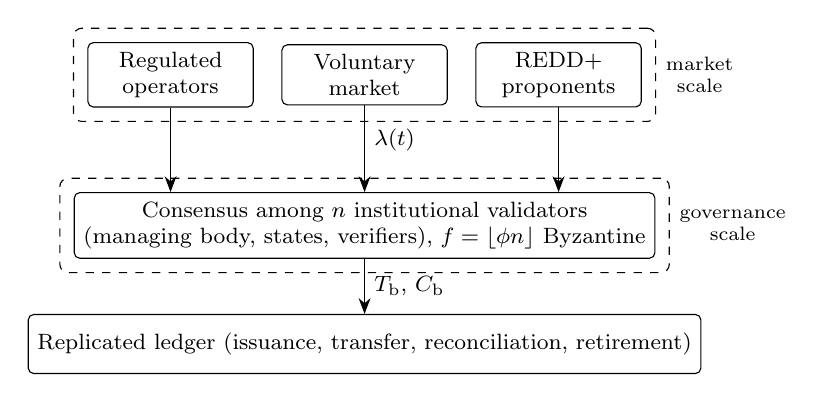
\begin{tikzpicture}[
  font=\footnotesize,
  box/.style={draw, rounded corners=2pt, align=center, minimum width=2.1cm, minimum height=0.75cm},
  layer/.style={draw, dashed, rounded corners=3pt, inner sep=5pt},
  >={Stealth[length=2mm]}]
  \node[box] (op) {Regulated\\operators};
  \node[box, right=0.35cm of op] (vol) {Voluntary\\market};
  \node[box, right=0.35cm of vol] (prop) {REDD+\\proponents};
  \node[box, below=1.1cm of vol, minimum width=6.8cm] (cons) {Consensus among $n$ institutional validators\\(managing body, states, verifiers), $f = \lfloor \phi n \rfloor$ Byzantine};
  \node[box, below=0.7cm of cons, minimum width=6.8cm] (led) {Replicated ledger (issuance, transfer, reconciliation, retirement)};
  \draw[->] (op) -- (op |- cons.north);
  \draw[->] (vol) -- node[right, pos=0.4]{$\lambda(t)$} (cons);
  \draw[->] (prop) -- (prop |- cons.north);
  \draw[->] (cons) -- node[right]{$\Tb$, $\Cb$} (led);
  \begin{scope}[on background layer]
   \node[layer, fit=(op)(vol)(prop), label={[font=\scriptsize,align=center]right:market\\scale}] {};
   \node[layer, fit=(cons), label={[font=\scriptsize,align=center]right:governance\\scale}] {};
  \end{scope}
\end{tikzpicture}}
\caption{Considered registry: the demand $\lambda(t)$ is determined by the market scale, whereas the cost of each consensus round is determined by the governance scale $n$.}
\label{fig:system}
\end{figure}

The separation between the two scales has a direct consequence. Let $B$ denote the number of transactions per block. The communication cost of consensus is incurred per block and is approximately independent of $B$, whereas the cost of disseminating the block content grows with $B$. Thus, the total traffic per block can be decomposed as
\begin{equation}
\Cb(n, B) \approx \underbrace{M(n)\, s_{\mathrm{v}}}_{\text{consensus}} + \underbrace{(n-1)\, B\, s_{\mathrm{tx}}}_{\text{dissemination}},
\label{eq:decomp}
\end{equation}
where $M(n)$ is the number of consensus messages per block, $s_{\mathrm{v}}$ is the size of a vote message and $s_{\mathrm{tx}}$ is the average transaction size. Expression \eqref{eq:decomp} indicates that the transaction volume mainly affects the second term, linear in $n$, while the potentially quadratic term depends only on governance. It also implies that $\Cb$ does not follow a single power law in $n$: the effective exponent varies between $1$ and $2$ according to the ratio between the two terms, which is taken into account in Section~\ref{sec:method}. The expression is treated as a hypothesis to be tested, not as a substitute for measurement.

\subsection{Demand Model of the National Registry}

Let $N_{\mathrm{op}}$ denote the number of active operators and participants, $\kappa$ the average number of registry transactions per participant in a compliance period of length $P$ (reports, transfers, reconciliations and retirements), and $\eta$ the fraction of these transactions that occurs within a window of length $\Delta$ preceding the reconciliation deadline. The mean and peak rates are given by
\begin{equation}
\bar{\lambda} = \frac{N_{\mathrm{op}}\,\kappa}{P}, \qquad \lambda_{\mathrm{peak}} = \frac{\eta\, N_{\mathrm{op}}\,\kappa}{\Delta},
\label{eq:demand}
\end{equation}
respectively, so that the peak-to-mean ratio is $\rho_{\mathrm{p}} = \eta P / \Delta$. This load is represented by a two-state Markov-modulated Poisson process (MMPP-2) \citep{Fischer1993}, whose high-activity state has a mean duration equal to the window and occurs, on average, once per period. In this manner, the MMPP-2 parameters are fully determined by
\begin{gather}
\frac{1}{\sigma_{2}} = \Delta, \qquad \frac{1}{\sigma_{1}} = P - \Delta, \nonumber\\
\lambda_{2} = \lambda_{\mathrm{peak}}, \qquad \lambda_{1} = \frac{(1-\eta)\,N_{\mathrm{op}}\,\kappa}{P - \Delta},
\label{eq:mmpp}
\end{gather}
where $\lambda_{1}$ and $\lambda_{2}$ are the rates in the low- and high-activity states and $1/\sigma_{1}$ and $1/\sigma_{2}$ are the respective mean sojourn times. It can be verified that the fraction of time in the high-activity state is $\sigma_{1}/(\sigma_{1}+\sigma_{2}) = \Delta/P$ and that the mean rate of the process,
\begin{equation}
\frac{\sigma_{2}\lambda_{1} + \sigma_{1}\lambda_{2}}{\sigma_{1} + \sigma_{2}} = \bar{\lambda},
\label{eq:meanrate}
\end{equation}
coincides with that of \eqref{eq:demand}. The load is concentrated only if $\eta > \Delta/P$, i.e., if $\rho_{\mathrm{p}} > 1$; for $\eta = \Delta/P$, the MMPP-2 reduces to a Poisson process. As a reference, a Poisson process with the same mean rate $\bar{\lambda}$ is used, which allows the effect of temporal concentration to be isolated from the effect of load intensity \citep{Paxson1995}.

Since the SBCE regulation is yet to define the covered sectors and the length of the compliance periods \citep{Lei15042}, the values of $N_{\mathrm{op}}$, $\kappa$, $\eta$, $\Delta$ and $P$ are not fixed in a single scenario. The mean rate is varied over three orders of magnitude, and the peak-to-mean ratio $\rho_{\mathrm{p}}$ is evaluated in a sensitivity experiment (Section~\ref{sec:method}). The feasibility frontiers are therefore presented as functions of $\bar{\lambda}$ for each evaluated value of $\rho_{\mathrm{p}}$, and not for an arbitrary regulatory scenario. \chk{Define the ranges of $N_{\mathrm{op}}$, $\kappa$, $\eta$, $\Delta$ and $P$ and their sources.}

\subsection{Metrics and Feasibility Criteria}

The considered metrics are the average block finalization time, $\Tb$, and the total traffic per block, $\Cb$, as in \citep{Caburlao2025reic,Caburlao2026clei}, complemented by the maximum traffic per node, $\Cn$, the sustained throughput, $\Th$, defined as the highest confirmation rate maintained under saturation, the 95th percentile of the transaction confirmation latency, $\Lt$, and the occupancy of the most loaded uplink, $\Ut$, measured as the fraction of time during which that link is busy. Since JABS models per-node send and receive queues, $\Ut$ is obtained directly from the simulation, and its analytical approximation,
\begin{equation}
\Ut \approx \frac{8\, \Cn\, \nu_{\mathrm{b}}}{\Kn},
\label{eq:util}
\end{equation}
where $\Cn$ is expressed in bytes per block, $\nu_{\mathrm{b}}$ is the block production rate and $\Kn$ is the link capacity in bits per second, is used only as a check. Unlike $\Cb$, the metric $\Ut$ captures the bottleneck node, which is essential for leader-centric protocols such as HotStuff.

A configuration is considered viable if it simultaneously meets three criteria, fixed before the main battery:
\begin{align}
\text{(V1) stability:} \quad & Q(kP) \leq \epsilon_{Q}\ \ \forall k, \nonumber\\
\text{(V2) latency:} \quad & \Lt \leq L_{\max}, \label{eq:feas}\\
\text{(V3) link:} \quad & \Ut \leq U_{\max}, \nonumber
\end{align}
where $Q(kP)$ is the number of pending transactions at the end of the $k$-th compliance period and $\epsilon_{Q}$ is a tolerance. Criterion V1 requires the backlog formed during the peak window to be drained before the next period, which is less restrictive than requiring $\Th \geq \lambda_{\mathrm{peak}}$, since short bursts can be absorbed by queueing. The effect of this queueing on users is captured by V2. The feasibility frontier of a protocol, $\nmax(\bar{\lambda})$, is the largest $n$ that meets \eqref{eq:feas} for a given demand, and the binding constraint is the first criterion violated as $n$ grows. \chk{Fix $\epsilon_{Q}$, $L_{\max}$ (e.g., as a fraction of $\Delta$) and $U_{\max}$ (e.g., $0.7$) before the main battery.}

% =====================================================================
\section{Methodology}
\label{sec:method}
% =====================================================================

\subsection{Experimental Design}

The experiments follow the methodology of \citet{Jain1991} and are organized in a pilot experiment, the fixing of the analysis protocol and the main battery. The pilot is used to validate the simulator, estimate the variability of the responses and determine the number of replications. The metrics, levels, tests, significance level, thresholds of \eqref{eq:feas} and the recommendation rule are registered before the main battery.

For transparency, it is noted that the design described here results from a revision of the initial study design, motivated by the identification of the traffic estimate discussed below and by questions on the scalability of pBFT at the national scale. The revision took place before the main battery, and the runs performed with the initial design are used only in the pilot. \chk{State whether any results from those runs were examined before the revision and how.}

The main battery comprises two experiments. Experiment E1 is a full factorial design with the factors in Table~\ref{tab:factors}, which include the fraction of Byzantine validators, so that the feasibility frontiers are also obtained under faults. The level $\phi = 0.30$ lies below the one-third threshold of all retained protocols; for $n = 4$, it corresponds to $f = 1$. Experiment E2 evaluates the sensitivity to demand concentration, with $\rho_{\mathrm{p}}$ at three levels, for the BFT protocols at the combinations of $n$ and $\bar{\lambda}$ closest to the frontiers obtained in E1. In addition, the levels $n \in \{400, 800\}$ are not used in any fit and serve exclusively to validate the metamodels, in a subset of cells of E1 (intermediate demand, institutional link); the level $n = 400$ coincides with the largest scale mentioned in the preliminary evaluation of Arq-REDD+ \chk{confirm}. The computational feasibility of the runs with $n = 800$, in which pBFT exchanges on the order of $10^{6}$ messages per block, is verified in the pilot.

\begin{table}[!ht]
\caption{Factors and levels of experiment E1 and their justification.}
\label{tab:factors}
\centering
\footnotesize
\setlength{\tabcolsep}{3pt}
\begin{tabular}{@{}lp{2.5cm}p{3.0cm}@{}}
\hline\hline
Factor & Levels & Justification \\
\hline
A: Protocol & pBFT, Tendermint, HotStuff, PoSA, PoS & Table~\ref{tab:req} \\
N: Validators $n$ & 4, 16, 64, 256 & governance range, ratio 4 \\
D: Demand $\bar{\lambda}$ & $\lambda_{0}$, $10\lambda_{0}$, $100\lambda_{0}$ & regulatory scenarios \eqref{eq:demand} \\
R: Regime & Poisson, MMPP-2 & concentration at deadlines \\
K: Link $\Kn$ & institutional, constrained & connectivity of remote nodes \\
$\Phi$: Byzantine $\phi$ & 0, 0.30 & requirement R3 \\
\hline
\multicolumn{2}{@{}l}{Configurations} & $5\times4\times3\times2\times2\times2 = 480$ \\
\hline\hline
\end{tabular}
\end{table}

All simulations are performed on the JABS simulator \citep{Yajam2023}. The current version of the simulator includes pBFT, PoSA (Parlia) and Casper FFG, with Poisson transaction arrivals; the execution of E1 requires the implementation of Tendermint, HotStuff, the MMPP-2 generator of \eqref{eq:mmpp} and the view changes of pBFT, without which a Byzantine leader halts the progress of the protocol. \chk{Conditional on these implementations and on their validation in the pilot.} Byzantine validators adopt silent behavior, i.e., they stop sending votes and, when leaders, stop proposing blocks \chk{confirm the attack types available in \texttt{ByzantineConfig}}.

One methodological aspect is decisive for the validity of the conclusions: the traffic $\Cb$ is measured at packet level, by summing the size of all messages actually exchanged to finalize each block, for all protocols. In the current version of the simulator, the traffic of pBFT is estimated as $2n \times 1{,}024$ bytes per block plus noise, which corresponds to a single node sending two 1~KiB messages to each of the others. In JABS, however, a pBFT vote has $42$ bytes ($32$ bytes of hash and $10$ bytes of overhead). Considering votes only, the expected total traffic is of the order of $2n^{2} \times 42$ bytes, so that the estimate overestimates the traffic for $n \lesssim 24$ and underestimates it for larger values, with a ratio of the order of $16$ at $n = 400$. \chk{Conditional on the acceptance and implementation of ADR-0001.} Each configuration is executed with $r$ independent replications, with distinct seeds and removal of the initial transient \citep{Law2015}, where $r$ is obtained from the pilot so that the half-width of the $95\%$ confidence interval of the stochastic responses does not exceed $5\%$ of the mean \citep{Jain1991}:
\begin{equation}
r = \max_{m}\left\lceil \left( \frac{z_{0.975}\, s_{m}}{0.05\, \bar{y}_{m}} \right)^{2} \right\rceil.
\label{eq:reps}
\end{equation}

Before the main battery, the simulator is validated in two steps. In the first, the scenarios of \citep{Caburlao2026clei} for PoSA and PoS are reproduced. In the second, it is verified that the number of consensus messages measured for pBFT with $n \in \{4, 16, 64\}$ matches the value expected from the protocol specification, which confirms the correctness of the instrumentation.

\subsection{Elasticities and Out-of-Range Validation}

The central question of this work, i.e., whether viability is more sensitive to the governance scale or to the market scale, is answered by elasticities, which are dimensionless and do not depend on the range of the chosen levels. For the total traffic, the two-term metamodel suggested by \eqref{eq:decomp},
\begin{equation}
\Cb = \alpha\, n^{\,b} + \beta\, (n-1)\, \bar{B},
\label{eq:cbmodel}
\end{equation}
is fitted by nonlinear least squares for each protocol and each combination of factors R, K and $\Phi$, where $\bar{B}$ is the measured average number of transactions per block and $b$ is the exponent of the consensus term, expected to be close to $2$ for pBFT and Tendermint and to $1$ for HotStuff in the normal case \eqref{eq:mpbft}. For $\Tb$, $\Lt$ and $\Ut$, the metamodel
\begin{multline}
\ln y = a + b \ln n + c \ln \bar{\lambda} + d \ln n \ln \bar{\lambda} \\
+ \textstyle\sum_{X \in \{R, K, \Phi\}} g_{X}\, \mathbb{1}_{X} + e
\label{eq:scaling}
\end{multline}
is fitted, where $\mathbb{1}_{X}$ are indicator variables of the levels of R, K and $\Phi$. The elasticities with respect to both scales are then
\begin{equation}
\varepsilon_{n} = \frac{\partial \ln y}{\partial \ln n}, \qquad \varepsilon_{\lambda} = \frac{\partial \ln y}{\partial \ln \bar{\lambda}},
\label{eq:elast}
\end{equation}
evaluated at the center of the governance and demand ranges, with confidence intervals obtained by bootstrapping over the replications. The metamodels are used to predict the responses at $n \in \{400, 800\}$ and are considered valid for extrapolation if the simulated values at these levels lie within the $95\%$ prediction intervals and the mean absolute percentage error is below $10\%$ \citep{Kleijnen2015}. \chk{Threshold to be fixed before the main battery.} For PoS and PoSA, $n$ represents the number of validators taking part in block production and finalization, and no theoretical expectations are formulated for the exponents.

\subsection{Tests of Effects by Analysis of Variance}

The ANOVA is used to test the existence of effects and, above all, of the interactions that determine whether the ranking of the protocols changes with the operating conditions. Since the factors are deliberately chosen, a fixed-effects model is adopted. For each stochastic response $m \in \{\Tb, \Lt, \Ut\}$, the observation $y$ of the $l$-th replication in cell $c$ of the design is modeled as
\begin{equation}
y^{(\theta)}_{cl} = \mu + \sum_{E \in \mathcal{E}} \tau_{E}(c) + \varepsilon_{cl},
\label{eq:anova}
\end{equation}
where $\mathcal{E}$ is the set of main and interaction effects among the factors in Table~\ref{tab:factors}, $\tau_{E}(c)$ is the effect $E$ in cell $c$, subject to sum-to-zero constraints, and $y^{(\theta)}$ is the Box--Cox transformation \citep{BoxCox1964},
\begin{equation}
y^{(\theta)} = \begin{cases} (y^{\theta}-1)/\theta, & \theta \neq 0, \\ \ln y, & \theta = 0, \end{cases}
\label{eq:boxcox}
\end{equation}
which is required because the responses are positive, skewed and vary over several orders of magnitude across protocols, which renders the effects multiplicative \citep{Jain1991,Montgomery2017}. The traffic $\Cb$ is not subjected to the ANOVA since, for the BFT protocols, the message count per block is practically deterministic and the variance across replications tends to zero, which would render the tests degenerate; for this response, the analysis relies exclusively on \eqref{eq:cbmodel}.

The analysis follows five steps: (i) $F$-tests for all effects, with coinciding sums of squares since the design is balanced; (ii) verification of the normality of the residuals through quantile--quantile plots, complemented by the Shapiro--Wilk test \citep{Shapiro1965} only in cells with up to $5{,}000$ observations, and of the homogeneity of variances through the Brown--Forsythe test \citep{Brown1974}; (iii) repetition of the inference with heteroscedasticity-consistent (HC3) standard errors \citep{Long2000} and with a nonparametric factorial analysis based on the aligned rank transform (ART) \citep{Wobbrock2011}, which preserves the tests of interactions, an effect being considered established only if significant in the three analyses; (iv) comparisons among protocols within each level of the factors with which they interact, by the Games--Howell procedure \citep{Games1976}, with family-wise error control by the Holm procedure \citep{Holm1979} at $\alpha = 0.05$; and (v) effect sizes through the statistic
\begin{equation}
\omega^{2}_{E} = \frac{SS_{E} - \mathit{df}_{E}\, MS_{\mathrm{err}}}{SST + MS_{\mathrm{err}}}
\label{eq:omega}
\end{equation}
\citep{Olejnik2003}. The shares of variation $SS_{E}/SST$ \citep{Jain1991} are reported descriptively and are not used to compare the importance of factors whose level ranges were fixed arbitrarily, a role that belongs to the elasticities \eqref{eq:elast}. No factor is discarded on the basis of a weak main effect alone when its interactions are significant.

\subsection{Feasibility Frontiers and Recommendation}

The frontiers $\nmax(\bar{\lambda})$ are obtained, for each protocol and each combination of $\rho_{\mathrm{p}}$, K and $\Phi$, by inverting the validated metamodels with respect to criteria \eqref{eq:feas}, and confirmed by direct simulation at points immediately below and above the estimated frontier. The protocol recommendation for a governance scenario $n$ and a demand $\bar{\lambda}$ follows three steps fixed before the main battery: (i) admissibility, which requires full compliance with R1--R4 and a tolerance threshold above $\phi$; (ii) feasibility by criteria \eqref{eq:feas}; and (iii) among the admissible and feasible protocols, preference for the lowest $\Lt$, since it is the metric perceived by the market participants, with ties, when confidence intervals overlap, broken by the largest margin $\nmax(\bar{\lambda})/n$, which favors configurations capable of accommodating the expansion of governance without re-engineering the registry.

% =====================================================================
\section{Numerical Results and Discussions}
\label{sec:results}
% =====================================================================

In this section, the numerical results of the main battery are presented along with the corresponding statistical analysis. All results are reported as means with $95\%$ confidence intervals over $r = $ \tbd{value} replications, and it is assumed that $\lambda_{0} = $ \tbd{value} transactions per second and $\rho_{\mathrm{p}} = $ \tbd{value}, unless otherwise stated.

\subsection{Simulator Validation and Effect of Traffic Measurement}

\begin{figure}[!ht]
\centering
\figplaceholder{4.5cm}{Fig. 2 -- pBFT $\Cb$ versus $n$ (log-log): closed-form estimate versus packet-level measurement, $n$ from 4 to 400, with the crossover point indicated.}
\caption{Block finalization traffic of pBFT versus the number of validators: closed-form estimate of the current simulator version and packet-level measurement.}
\label{fig:artifact}
\end{figure}

\tbd{Outcome of the reproduction of the scenarios of \citep{Caburlao2026clei} for PoSA and PoS and of the pBFT message count check.} Fig.~\ref{fig:artifact} compares, for pBFT, the closed-form estimate with the traffic measured at packet level. It can be seen that \tbd{describe: the estimate grows with exponent 1, whereas the measurement grows with exponent $\hat{b} = $ ...; locate the crossover, expected close to $n = 24$}. This is expected since the estimate assumes 1~KiB messages sent by a single node, whereas the measurement sums $42$-byte votes exchanged in two all-to-all phases \eqref{eq:mpbft}. Therefore, the estimate misses not only the absolute value but also the shape of the growth, which is what determines viability at scale.

\subsection{Scaling Laws and Elasticities}

\begin{figure}[!ht]
\centering
\figplaceholder{4.5cm}{Fig. 3 -- $\Cb$ and $\Cn$ versus $n$ (log-log) for the five protocols, with fits of \eqref{eq:cbmodel} and validation points at 400 and 800.}
\caption{Total traffic per block and maximum traffic per node versus the number of validators, with the fitted metamodels and the validation points outside the fitting range.}
\label{fig:scaling}
\end{figure}

Fig.~\ref{fig:scaling} shows the total traffic and the traffic of the most loaded node as functions of $n$. It can be seen that \tbd{estimated exponents $\hat{b}$ of the consensus term per protocol and comparison with theory}. In particular, \tbd{HotStuff: total traffic exponent close to 1, but leader traffic also linear in $n$; discuss whether the leader becomes the bottleneck}. The validation points at $n \in \{400, 800\}$ \tbd{do/do not lie within the prediction intervals; MAPE}.

\begin{table}[!ht]
\caption{Elasticities with respect to governance ($\varepsilon_{n}$) and demand ($\varepsilon_{\lambda}$), evaluated at the center of the ranges, with $\phi = 0$ and institutional link (\textcolor{red}{?}: pending).}
\label{tab:elast}
\centering
\footnotesize
\setlength{\tabcolsep}{3pt}
\begin{tabular}{@{}lcccccc@{}}
\hline\hline
\multirow{2}{*}{Protocol} & \multicolumn{2}{c}{$\Cb$} & \multicolumn{2}{c}{$\Lt$} & \multicolumn{2}{c}{$\Ut$} \\
 & $\varepsilon_{n}$ & $\varepsilon_{\lambda}$ & $\varepsilon_{n}$ & $\varepsilon_{\lambda}$ & $\varepsilon_{n}$ & $\varepsilon_{\lambda}$ \\
\hline
pBFT       & \tbdc & \tbdc & \tbdc & \tbdc & \tbdc & \tbdc \\
Tendermint & \tbdc & \tbdc & \tbdc & \tbdc & \tbdc & \tbdc \\
HotStuff   & \tbdc & \tbdc & \tbdc & \tbdc & \tbdc & \tbdc \\
PoSA       & \tbdc & \tbdc & \tbdc & \tbdc & \tbdc & \tbdc \\
PoS        & \tbdc & \tbdc & \tbdc & \tbdc & \tbdc & \tbdc \\
\hline\hline
\end{tabular}
\end{table}

Table~\ref{tab:elast} presents the elasticities. \tbd{Compare $\varepsilon_{n}$ and $\varepsilon_{\lambda}$ per protocol and response: this is the central evidence for the working hypothesis.}

\subsection{Binding Constraint and Feasibility Frontiers}

\begin{figure}[!ht]
\centering
\figplaceholder{5cm}{Fig. 4 -- $\nmax$ versus $\bar{\lambda}$ (log-log) for each protocol, link and $\phi$; governance range ($n \le 256$) shaded; marker indicating the binding constraint (V1, V2 or V3).}
\caption{Feasibility frontiers $\nmax(\bar{\lambda})$ for each protocol, link capacity and Byzantine fraction, with the governance range highlighted and the binding constraint indicated.}
\label{fig:frontier}
\end{figure}

Fig.~\ref{fig:frontier} illustrates the feasibility frontiers. \tbd{For each protocol: at which demand the frontier crosses the governance range; which criterion is exhausted first; shift of the frontier with $\phi = 0.30$ and with the constrained link.} \tbd{Relation between the frontier and the territorial sizing ($n \approx 10^5$).}

\subsection{Effect of Demand Concentration}

\tbd{Experiment E2: shift of $\Lt$ and of $\nmax$ with $\rho_{\mathrm{p}}$; compare with Poisson at the same $\bar{\lambda}$ and discuss whether a Poisson-based evaluation would overestimate the frontier.}

\subsection{Tests of Effects and Interactions}

\begin{table*}[!ht]
\caption{Effects and interactions of the stochastic responses of E1: $p$-values of the classical and ART analyses and effect size $\omega^{2}_{E}$. Only effects significant in the three analyses (classical, HC3 and ART) are shown.}
\label{tab:anova}
\centering
\small
\begin{tabular}{@{}lccccccccc@{}}
\hline\hline
\multirow{2}{*}{Effect} & \multicolumn{3}{c}{$\Tb$} & \multicolumn{3}{c}{$\Lt$} & \multicolumn{3}{c}{$\Ut$} \\
 & $p_{F}$ & $p_{\mathrm{ART}}$ & $\omega^{2}_{E}$ & $p_{F}$ & $p_{\mathrm{ART}}$ & $\omega^{2}_{E}$ & $p_{F}$ & $p_{\mathrm{ART}}$ & $\omega^{2}_{E}$ \\
\hline
A$\times$N        & \tbdc & \tbdc & \tbdc & \tbdc & \tbdc & \tbdc & \tbdc & \tbdc & \tbdc \\
A$\times$R        & \tbdc & \tbdc & \tbdc & \tbdc & \tbdc & \tbdc & \tbdc & \tbdc & \tbdc \\
A$\times\Phi$     & \tbdc & \tbdc & \tbdc & \tbdc & \tbdc & \tbdc & \tbdc & \tbdc & \tbdc \\
A$\times$K        & \tbdc & \tbdc & \tbdc & \tbdc & \tbdc & \tbdc & \tbdc & \tbdc & \tbdc \\
D$\times$R        & \tbdc & \tbdc & \tbdc & \tbdc & \tbdc & \tbdc & \tbdc & \tbdc & \tbdc \\
\hline\hline
\end{tabular}
\end{table*}

Table~\ref{tab:anova} presents the established effects and interactions. \tbd{Box--Cox $\hat\theta$; assumption checks; agreement among the three analyses (report $p_{\mathrm{HC3}}$ in the text or in supplementary material).} \tbd{Discuss under which conditions the ranking of the protocols is reversed (interactions with A).}

\subsection{Discussion: National-Scale Viability}

\tbd{Answer directly, based on the frontiers, whether Byzantine consensus is viable at national scale: (a) with institutional governance ($n \le 256$), which protocols are viable for each demand range, with and without Byzantine validators; (b) with territorial sizing, whether any flat Byzantine protocol is viable or whether the alternative is a hierarchical architecture \citep{Amir2010}; (c) implications for the regulation of the SBCE central registry.}

\subsection{Limitations}

\tbd{Simulation-based evaluation; parametric demand until the SBCE regulation; a single Byzantine behavior (silence); security assessment restricted to the tolerance threshold; hierarchical architectures discussed but not simulated; smart contract and oracle risks out of scope \citep{GhiyamiPour2025,Rahman2023}.}

% =====================================================================
\section{Conclusions}
\label{sec:conclusion}
% =====================================================================

This contribution investigated the viability of Byzantine consensus for a national blockchain-based carbon credit registry. The question was formulated in terms of two distinct scales: the governance scale, which determines the number of validators and the communication cost of each consensus round, and the market scale, which determines the transaction demand and its concentration around reconciliation deadlines. The evaluated protocols were selected from domain requirements, consensus traffic was measured at packet level, Byzantine validators were included in the factorial design, and the elasticities with respect to both scales were estimated by metamodels validated outside the fitting range, with interactions tested by ANOVA. It was shown that \tbd{main finding on elasticities and binding constraint} and that \tbd{feasibility frontiers within the governance range, with and without faults}, which \tbd{confirms/refutes} the hypothesis that the viability of a national registry depends more on its governance design than on its transaction volume. In either case, the resulting frontiers can inform the regulation of the SBCE central registry by making explicit how many validators a registry can accommodate for each demand level. Possible future extensions of this work involve the simulation of hierarchical consensus architectures, the inclusion of other Byzantine behaviors and the calibration of the demand model with data from the first SBCE compliance periods. Another direction of research could investigate the impact of MRV oracles on the demand and security of the registry.

% =====================================================================
\begin{declarations}

\begin{acknowledgements}
\chk{Optional.}
\end{acknowledgements}

\begin{contributions}
\chk{CRediT statement to be defined by the authors; suggestion to be confirmed: FRF contributed to the conception of this study, the experimental design and the statistical analysis. MCC developed the Arq-REDD+ architecture and the simulation scenarios. CKSR supervised the work. All authors read and approved the final manuscript.}
\end{contributions}

\begin{interests}
The authors declare that they have no competing interests.
\end{interests}

\begin{materials}
The simulator and the scripts used in the current study are available at \url{https://github.com/frfreire/Arq-REDD-Framework}. \chk{Add the dataset and registered analysis protocol link (e.g., OSF or Zenodo DOI).}
\end{materials}

\begin{funding}
\chk{Optional.}
\end{funding}

\begin{furtherinformation}
This research did not involve human participants and, therefore, did not require approval by an ethics committee. \chk{Declare the use of generative AI tools, if applicable.}
\end{furtherinformation}

\end{declarations}

\bibliographystyle{apalike-sol}
\bibliography{refs}

\end{document}
